%本章探讨改进失效现象

\chapter{改进失效现象}

在第\ref{chapter:优化潜力}章的证明过程中,我们通过添加项的方式对不等式进行放缩,从而证明了$\sum_{i=1}^N\xi_i > \xi$是严格成立的。但是这一推导过程中,我们默认了$z_\eta>0$。由$z_\eta$的定义可知
\[
z_\eta>0 \Longleftrightarrow \eta > 0.5
\]
也就是说,只有当企业设定的服务水平高于50\%时,才能够通过保留在制品库存降低企业库存总量。

当$\eta=0.5$时,有$z_\eta=0$,参考公式\ref{eq:改进前后库存比较i}的推导过程,可知此时$\sum_{i=1}^N\xi_i - \xi = 0$,即改进前后企业的总库存没有发生变化。

当$\eta<0.5$时,有$z_\eta<0$,参考公式\ref{eq:改进前后库存比较i}的推导过程,可以发现此时的不等式放缩方向是相反的,应该得到$\sum_{i=1}^N\xi_i - \xi < 0$,即改进后反而使得企业的总库存增加。

由此可见,当需求服从正态分布时,在某些服务水平下,将成品库存合并前移到在制品库存不仅没有起到改进效果,反而会使总库存增大。我们将这种情况称为改进失效。

本章将结合常用的需求分布函数,详细讨论改进失效现象与需求分布、服务水平等因素的关系。







\section{对称稳定分布的参数与改进失效的关系}

前面的部分主要考虑了需求为正态分布时,改进策略对库存总量的影响。之所以研究正态分布,是因为正态分布确实广泛存在于现实生活中。实际生产中的需求分布可能是各种各样的,甚至可能写不出解析式,但只要是方差有限的独立同分布,根据中心极限定理,在进行叠加的时候总会趋近于正态分布。而正态分布自身叠加仍是正态分布。因此,正态分布就像一个吸引域,从各种分布出发最终都落入正态分布。正态分布下的库存改进效果,也能在很大程度上反应实际的改进效果。

第\ref{chapter:优化潜力}章中已经提到,安全库存等于总库存与需求期望值之差。回顾公式\ref{eq:成品库存i}和\ref{eq:在制品库存i}可知,改进前和改进后的安全库存分别为$z_{\eta}\sum_{i=1}^n\sigma_i$和$z_\eta\sqrt{\sum_{i=1}^n\sigma_i^2}$。为了使考虑的问题更简单,我们假设所有的需求是独立同分布的$N(\mu,\sigma^2)$,则改进前和改进后的安全库存分别为$nz_\eta\sigma$和$\sqrt{n}z_\eta\sigma$。

当$\eta<0.5$的时候,安全库存是负值,这是实际生产中一般不会出现的情况。当$\eta>0.5$时,可以看到,$n$种成品合并之后的安全库存是单个成品安全库存的$\sqrt{n}$倍,而不合并的情况下则是单个成品的$n$倍。此时改进是一定有效果的。

事实上,像正态分布这种“合并后安全库存是单个成品安全库存的$n^{1/\alpha}$倍”的性质,还出现在其他的对称稳定分布中。Feller(2008)\cite{feller_introduction_2008}提到,对称稳定分布有$f_{n,\alpha}(x)=f_\alpha(n^{1/\alpha}x)$的性质。也就是说,$n$个独立同分布的对称稳定分布的随机变量$X$相加,和的概率分布与随机变量$n^{1/\alpha}X$是相同的。而正态分布正是对称稳定分布取$\alpha=2$的一个特例。

稳定分布的概率密度函数为$f(x;\alpha,\beta,c,\mu)$,其中参数$\alpha\in(0,2]$,影响曲线的陡峭程度;$\beta\in[-1,1]$,影响曲线的偏斜程度;$c\in(0,+\infty)$,影响曲线的水平尺度;$\mu\in(-\infty,+\infty)$,影响曲线的水平中心。当$\beta=0$时,即为对称稳定分布。图
\ref{fig:对称稳定分布}展示了$\beta=0,c=1,\mu=0$的对称稳定分布在不同的$\alpha$取值下的图形,其中$\alpha=2$时即为正态分布。

\begin{figure}[htb]
\centering
\includegraphics[width=15cm]{stable.eps}
\caption{不同参数$\alpha$下的对称稳定分布}
\label{fig:对称稳定分布}
\end{figure}

广义中心极限定理指出,$n$个独立同分布的随机变量(方差可以无限)相加,最终会收敛到一个稳定分布。因此,和正态分布一样,稳定分布也广泛存在于实际生活中。Newman(2005)\cite{newman_power_2005}的一系列实证分析证实了这一点。

假设单个成品需求服从对称稳定分布$f(x;\alpha,0,c,\mu)$,则它的安全库存服从对称稳定分布$f(x;\alpha,0,c,0)$。设此需求分布下,满足服务水平$\eta$需要的安全库存为$s$,$n$个成品需要的总安全库存是$ns$。根据(Feller)所述的性质可以推知,改进后需要的安全库存为$n^{1/\alpha}s$。$\eta>0.5$时$s>0$,故改进是否有效就取决于$\alpha$的取值。将改进前后的库存作比较:
\[
\frac{ns}{n^{1/\alpha}s} = n^{1-1/\alpha}
\]
其中$\alpha$的取值范围是$(0,2]$。

当$\alpha\in(1,2]$时,$n^{1-1/\alpha}>1$,改进前的库存大于改进后的库存,改进有效。

当$\alpha\in(0,1]$时,$n^{1-1/\alpha}\leq 1$,改进前的库存不大于改进后的库存,改进无效。









\section{右偏斜的需求分布一定存在改进失效的可能}

对称分布存在一个普遍的缺点——需求可能出现负值,因此我们在实际生产中也常常使用一些其他的分布函数来描述需求的分布。现实的需求不可能为负值,其概率密度函数一般不会有左侧的长尾。因此,需求分布一般都是右偏斜的。Agrawal和Smith(1996)\cite{agrawal_estimating_1996}使用一些实际的需求数据,拟合一些常用的需求分布,包括泊松分布、指数分布、负二项分布等。它们都是右偏斜的分布。

假设有$n$种颜色的成品,其需求$D_i(i=1,2,\ldots,n)$独立同分布且该分布是右偏斜的,累积分布函数都为$F$,均值为$\mu$,方差为$\sigma^2$。将成品库存合并前移到在制品库存后,在制品的总需求为$D_n=\sum_{i=1}^nD_i$,其累积分布函数为$F_n$,均值为$n\mu$,方差为$n\sigma^2$。

设每种颜色的成品库存量为$s$,则对应的服务水平为$\eta=F(s)$。由$F_n$的定义知
\begin{equation}
F_n(ns) = P(D_n<ns) = P\left(\frac{\sum_{i=1}^nD_i}{n}<s\right)
\label{eq:Fn转为均值形式}
\end{equation}

根据中心极限定理,当$n\to\infty$时,$\frac{1}{n}\sum_{i=1}^nD_i$的分布趋近于正态分布$N(\mu,\sigma^2/n)$。设正态分布$N(\mu,\sigma^2/n)$的累积分布函数为$G$。由中心极限定理得
\begin{equation}
\lim_{n\to\infty}P\left(\frac{\sum_{i=1}^nD_i}{n}<s\right) = \lim_{n\to\infty}\Phi\left(\frac{s-\mu}{\sigma/\sqrt{n}}\right) = \lim_{n\to\infty}G(s)
\label{eq:中心极限定理}
\end{equation}
其中$\Phi$为标准正态分布的累积分布函数。由公式\ref{eq:Fn转为均值形式}和\ref{eq:中心极限定理}可知
\begin{equation}
\lim_{n\to\infty}[F_n(ns)-G(s)]=0
\label{eq:Fn与G的极限形式}
\end{equation}

接下来我们将证明,对任何的右偏斜需求分布,一定存在一个区间,当服务水平在此区间内时,就存在改进失效的可能。已知需求$D_i$的分布是右偏的,因此有
\begin{equation}
F(\mu) > 0.5 = \Phi(0) = G(\mu)
\label{eq:右偏斜的性质}
\end{equation}
由$F$和$G$的连续性,至少存在一个$\mu$的领域$[\mu,s_0)$,使得这个区间内的所有库存值$s$都满足
\[
F(s) > G(s),\qquad \forall s\in[\mu,s_0)
\]
令$\delta=F(s)-G(s)>0$。在公式\ref{eq:Fn与G的极限形式}中,根据极限的定义,存在一个正数$N$,使得对任意的$n>N$,都有
\begin{equation}
|F_n(ns)-G(s)| < \delta = F(s) - G(s)
\label{eq:根据极限的定义}
\end{equation}
公式\ref{eq:根据极限的定义}显示,对于任意的$s\in[\mu,s_0)$,都存在一个$N$,使得$n>N$时恒有$F_n(ns)<F(s)$。

我们知道$F(s)$代表需求量小于$s$的概率,即库存量$s$对应的服务水平。反过来,某个服务水平$\eta$也对应着一个库存量,我们将这个对应关系定义为函数$F^{-1}$。函数$F^{-1}$的表达式为
\[
F^{-1}(\eta) = \inf\left\{s\middle|F(s)\geq\eta\right\}
\]
其中$\inf$表示集合的下确界。同理可定义$F_n^{-1}$。

若企业需要满足的服务水平为$\eta$,则改进前和改进后的库存分别为$F^{-1}(\eta)$和$F_n^{-1}(\eta)$。若改进后的在制品库存大于改进前的各颜色成品库存之和,就说明改进失效了。也就是说,改进失效的具体表现是$F_n^{-1}(\eta)>nF^{-1}(\eta)$。下面我们将证明,当$F^{-1}(\eta)\in[\mu,s_0)$时,存在改进失效的可能。

现在假设企业的设定的服务水平为$\eta$,满足$\eta\in[F(\mu),F(s_0))$,则改进前各颜色成品的库存为$s=F^{-1}(\eta)\in[\mu,s_0)$。前面已经证明,对于任意的$s\in[\mu,s_0)$,都存在一个$N$,使得$n>N$时恒有
\begin{equation}
F_n(ns)<F(s)=\eta
\label{eq:改进前后服务水平的关系}
\end{equation}
根据反函数的性质,由于累积分布函数$F$和$F_n$是单调递增的,所以$F^{-1}$和$F_n^{-1}$也是单调递增的。公式\ref{eq:改进前后服务水平的关系}显示$F_n(ns)<\eta$,结合$F_n^{-1}$的单调性可知
\begin{equation}
F_n^{-1}(\eta) > ns
\label{eq:反函数单调性}
\end{equation}
把$s=F^{-1}(\eta)$代入公式\ref{eq:反函数单调性}有
\[
F_n^{-1}(\eta)>nF^{-1}(\eta)
\]
前面已经提到,上式即为改进失效的具体表现。

通过本节的分析,我们证明了,当各颜色成品需求服从独立同分布的任意一种右偏斜分布时,存在一个大于$F^{-1}(\mu)$的服务水平区间,企业的服务水平位于这个区间时,存在改进失效的可能。当服务水平小于$F^{-1}(\mu)$时,安全库存是负值,无需过多讨论。







\section{任何服务水平都存在改进失效的可能}

在上一节的讨论中,我们已经证明,如果需求服从独立同分布的右偏斜分布,则存在一个大于$F^{-1}(\mu)$的服务水平区间,使得这个区间内的服务水平下可能发生改进失效的风险。那么,这个区间是否存在上限?当服务水平远高于$F^{-1}(\mu)$的时候,是否存在某些服务水平,使得在这些服务水平下一定不会发生改进失效?我们以最简单的伯努利分布为例,来研究这个问题。

如果单个产品的需求服从伯努利分布:需求量为$d_1$的概率为$\alpha$,需求量为$d_2$的概率为$1-\alpha$。为了保证需求是右偏的,我们设定$d_1 < d_2$,且$\alpha > 0.5$。

假设有两种颜色的成品,需求相互独立,且都服从上述的伯努利分布。企业的服务水平为$\eta$,则$\eta$和$\alpha$的相对大小会对库存产生影响:当$\eta > \alpha$时,每种成品需要保留的库存为$d_2$,总库存为$2d_2$;当$\eta \leq \alpha$时,每种成品需要保留的库存为$d_1$,总库存为$2d_1$。因此,改进前的服务水平与库存的关系如表\ref{tab:改进前服务水平与库存的关系_伯努利}所示。

\begin{table}[h]
\caption{改进前服务水平与库存的关系}
\label{tab:改进前服务水平与库存的关系_伯努利}
\begin{tabularx}{\textwidth}{YYY}
\toprule
服务水平 & 单个成品库存 & 总库存 \\
\midrule
$\eta > \alpha$ & $d_2$ & $2d_2$ \\
$\eta \leq \alpha$ & $d_1$ & $2d_1$ \\
\bottomrule
\end{tabularx}
\end{table}

现将这两种成品的库存合并保留到在制品库存。首先计算这两种成品需求的联合分布

\begin{table}[h]
\caption{两种成品需求的联合分布}
\label{tab:两种成品需求的联合分布_伯努利}
\begin{tabularx}{\textwidth}{YYY}
\toprule
第一种成品需求 & 第二种成品需求 & 概率 \\
\midrule
$d_1$ & $d_1$ & $\alpha^2$ \\
$d_1$ & $d_2$ & $\alpha(1-\alpha)$ \\
$d_2$ & $d_1$ & $\alpha(1-\alpha)$ \\
$d_2$ & $d_2$ & $(1-\alpha)^2$ \\
\bottomrule
\end{tabularx}
\end{table}


由表\ref{tab:两种成品需求的联合分布_伯努利}可以得到合并后在制品的需求分布,如表\ref{tab:在制品需求分布_伯努利}所示。

\begin{table}[h]
\caption{在制品需求分布}
\label{tab:在制品需求分布_伯努利}
\begin{tabularx}{\textwidth}{YYY}
\toprule
需求量 & 概率 & 累积概率 \\
\midrule
$2d_1$ & $\alpha^2$ & $\alpha^2$ \\
$d_1+d_2$ & $2\alpha(1-\alpha)$ & $2\alpha-\alpha^2$ \\
$2d_2$ & $(1-\alpha)^2$ & $1$ \\
\bottomrule
\end{tabularx}
\end{table}

企业的服务水平仍为$\eta$,根据表\ref{tab:在制品需求分布_伯努利}在制品的需求累积概率分布与$\eta$的相对大小,可以得出需要保留的在制品库存:当$\eta > 2\alpha - \alpha^2$时,在制品需要保留的库存为$2d_2$;当$\alpha^2 < \eta \leq 2\alpha - \alpha^2$时,在制品需要保留的库存为$d_1+d_2$;当$\eta \leq \alpha^2$时,在制品需要保留的库存为$2d_1$。因此,改进后的服务水平与库存的关系如表\ref{tab:改进后服务水平与库存的关系_伯努利}所示。

\begin{table}[h]
\caption{改进后服务水平与库存的关系}
\label{tab:改进后服务水平与库存的关系_伯努利}
\begin{tabularx}{\textwidth}{YYY}
\toprule
服务水平 & 在制品库存 \\
\midrule
$\eta > 2\alpha - \alpha^2$ & $2d_2$ \\
$\alpha^2 < \eta \leq 2\alpha - \alpha^2$ & $d_1+d_2$ \\
$\eta \leq \alpha^2$ & $2d_1$ \\
\bottomrule
\end{tabularx}
\end{table}

对比表\ref{tab:改进前服务水平与库存的关系_伯努利}和表\ref{tab:改进后服务水平与库存的关系_伯努利}可知:当$\eta \leq \alpha^2$时,改进前后的库存都为$2d_1$;当$\alpha^2 < \eta \leq \alpha$时,改进后的库存$2d_2$大于改进前的库存$2d_1$;$\alpha < \eta \leq 2\alpha - \alpha^2$时,改进后的库存$d_1+d_2$小于改进前的库存$2d_2$;当$\eta > 2\alpha - \alpha^2$时,改进前后的库存都为$2d_2$。汇总如表\ref{tab:不同服务水平下改进前后库存对比_伯努利}所示。

\begin{table}[h]
\caption{不同服务水平下改进前后库存对比}
\label{tab:不同服务水平下改进前后库存对比_伯努利}
\begin{tabularx}{\textwidth}{YYY}
\toprule
服务水平 & 改进前库存量 & 改进后库存量 \\
\midrule
$\eta \leq \alpha^2$ & $2d_1$ & $2d_1$ \\
$\alpha^2 < \eta \leq \alpha$ & $2d_1$ & $2d_2$ \\
$\alpha < \eta \leq 2\alpha - \alpha^2$ & $2d_2$ & $d_1+d_2$ \\
$\eta > 2\alpha - \alpha^2$ & $2d_2$ & $2d_2$ \\
\bottomrule
\end{tabularx}
\end{table}

从表\ref{tab:不同服务水平下改进前后库存对比_伯努利}中可以看出,当$\alpha^2 < \eta \leq \alpha$时,一定会发生改进失效。显然,对任意的服务水平$\eta$,一定存在某些$\alpha$,使得$\alpha^2 < \eta \leq \alpha$。因此,任意的服务水平下都能够找到某些右偏斜的伯努利分布,使得改进失效。

上述结论很容易推广到三种以上成品合并库存的情况。假设有$n$种颜色的成品,需求服从独立同分布的伯努利分布,需求量为$d_1$的概率为$\alpha$,需求量为$d_2$的概率为$1-\alpha$,$d_1 < d_2$,$\alpha > 0.5$。易知,当服务水平$\eta \leq \alpha$时,需要保留的单个成品库存量为$d_1$,总库存量为$nd_1$。将它们的库存合并到在制品库存后,在制品的需求服从二项分布,即
\[
P(kd_1+(n-k)d_2) = C_{n}^{k}\alpha^k(1-\alpha)^{n-k}
\]
取$k=n$可知$P(nd_1)=\alpha^n$,因此当服务水平$\eta > \alpha^n$时,需要保留的在制品库存量是大于$nd_1$的。当服务水平满足$\alpha^n < \eta \leq \alpha^n$时,一定发生改进失效。

通过以上讨论我们证明了,将$n$种颜色的成品库存合并为在制品库存时,对于任意的服务水平$\eta$,都可能在某些右偏的需求分布下发生改进失效。因此,企业在做出决策之前不能盲目乐观,必须根据自身的服务水平和实际的需求分布,谨慎地进行模拟和推算,防止发生改进失效。








\section{泊松分布下发生改进失效的区间图示}

在前两节的讨论中,我们从理论上证明了改进失效现象的存在性。但是,对改进失效现象发生的具体范围和如何避免,仍然没有清晰直观的认识。本节中,我们将以实际生产中常用的泊松分布为例,展示改进失效的实际影响和避免改进失效的方法。

为了精确描述库存总量在改进前后的变化,我们首先需要知道改进前后需求分布的变化。设需求$D$服从泊松分布$Po(\lambda)$,则其概率为
\[
P(D=x) = \frac{e^{-\lambda}\lambda^x}{x!},\qquad x\in\mathbb{N}
\]

设企业的服务水平为$\eta$,满足此服务水平所需的库存为$\xi$。则库存$\xi$的表达式为
\begin{equation}
\xi = \inf\left\{\xi\in\mathbb{N}\middle|\sum_{x=0}^{\xi}\frac{e^{-\lambda}\lambda^x}{x!}\geq \eta\right\}
\end{equation}
其中符号$\inf$表示集合的下确界。

设两种颜色的成品需求服从相互独立的泊松分布$Po(\lambda_1)$、$Po(\lambda_2)$。企业的服务水平为$\eta$。则两种成品需要保持的库存$\xi_1$、$\xi_2$分别为
\begin{align}
\xi_1 &= \inf\left\{\xi_1\in\mathbb{N}\middle|\sum_{x=0}^{\xi_1}\frac{e^{-\lambda_1}\lambda_1^x}{k!}\geq \eta\right\} \label{eq:成品库存_泊松1}\\
\xi_2 &= \inf\left\{\xi_2\in\mathbb{N}\middle|\sum_{x=0}^{\xi_2}\frac{e^{-\lambda_2}\lambda_2^x}{k!}\geq \eta\right\} \label{eq:成品库存_泊松2}
\end{align}

现在假设取消两种颜色的成品库存,改为保留共同的在制品库存。企业的服务水平仍然为$\eta$。为了满足该服务水平,所需的在制品库存为$\xi$。此时的在制品库存需要同时应对两种颜色的成品需求,因此,对未喷涂的在制品需求为$D=D_1+D_2$。

设$D_1$、$D_2$的联合分布为$f(x_1,x_2)$。因为$D_1$、$D_2$是独立的,所以$f(x_1,x_2)$的概率分布为
\begin{align}
f(x_1,x_2) &= f(x_1)f(x_2) \notag\\
&= \frac{e^{-\lambda_1}\lambda_1^{x_1}}{x_1!} \cdot \frac{e^{-\lambda_2}\lambda_2^{x_2}}{x_2!} \notag\\
&= \frac{e^{-(\lambda_1+\lambda_2)}\lambda_1^{x_1}\lambda_2^{x_2}}{x_1!x_2!}
\label{eq:联合分布_泊松}
\end{align}

设$D$、$D_2$的联合分布为$g(y_1,y_2)$。由$y_1=x_1+x_2,y_2=x_2$得$x_1=y_1-y_2,x_2=y_2$。与正态分布下的证明过程类似,我们求出雅可比矩阵
\[
J = \begin{bmatrix}
\frac{\partial x_1}{\partial y_1} & \frac{\partial x_1}{\partial y_2} \\
\frac{\partial x_2}{\partial y_1} & \frac{\partial x_2}{\partial y_2}
\end{bmatrix} = \begin{bmatrix}
1 & -1 \\
0 & 1
\end{bmatrix}
\]
由此可得$g(y_1,y_2)$的概率分布为
\begin{align}
g(y_1,y_2) &= f(y_1-y_2,y_2)\cdot\left|J\right| \notag\\
&= \frac{e^{-(\lambda_1+\lambda_2)}\lambda_1^{y_1-y_2}\lambda_2^{y_2}}{(y_1-y_2)!y_2!}
\label{eq:新联合分布_泊松}
\end{align}
然后求边缘分布$h(y_1)$。与前面不同的是,泊松分布的自变量$y_1-y_2\geq 0$,因此有$y_2\leq y_1$。
\begin{align}
h(y_1) &= \sum_{y_2=0}^{y_1}g(y_1,y_2) = \sum_{y_2=0}^{y_1}\frac{e^{-(\lambda_1+\lambda_2)}\lambda_1^{y_1-y_2}\lambda_2^{y_2}}{(y_1-y_2)!y_2!} \notag\\
&= \frac{e^{-(\lambda_1+\lambda_2)}(\lambda_1+\lambda_2)^{y_1}}{y_1!}\sum_{y_2=0}^{y_1}\frac{y_1!}{y_2!(y_1-y_2)!}\left(\frac{\lambda_1}{\lambda_1+\lambda_2}\right)^{y_1-y_2}\left(\frac{\lambda_2}{\lambda_1+\lambda_2}\right)^{y_2}
\label{eq:求边缘分布_泊松}
\end{align}
公式\ref{eq:求边缘分布_泊松}的右半部分是二项分布$B(y_1,\frac{\lambda_2}{\lambda_1+\lambda_2})$的全部累积概率,其和应该为1,即
\[
\sum_{y_2=0}^{y_1}\frac{y_1!}{y_2!(y_1-y_2)!}\left(\frac{\lambda_1}{\lambda_1+\lambda_2}\right)^{y_1-y_2}\left(\frac{\lambda_2}{\lambda_1+\lambda_2}\right)^{y_2} = 1
\]
因此得到边缘分布为
\begin{equation}
h(y_1) = \frac{e^{-(\lambda_1+\lambda_2)}(\lambda_1+\lambda_2)^{y_1}}{y_1!}
\label{eq:边缘分布结果_泊松}
\end{equation}

由公式\ref{eq:边缘分布结果_泊松}可知,在制品的总需求$D$服从泊松分布$Po(\lambda_1+\lambda_2)$。所以应保留的在制品库存为
\begin{equation}
\xi = \inf\left\{\xi\in\mathbb{N}\middle|\sum_{x=0}^{\xi}\frac{e^{-(\lambda_1+\lambda_2)}(\lambda_1+\lambda_2)^x}{x!}\geq \eta\right\}
\label{eq:在制品库存_泊松}
\end{equation}

根据公式\ref{eq:成品库存_泊松1}、\ref{eq:成品库存_泊松2}和\ref{eq:在制品库存_泊松},如果改进前的需求分布服从$Po(\lambda_1)$和$Po(\lambda_2)$,则改进后的需求服从$Po(\lambda_1+\lambda_2)$。据此,我们就可以算出各种情况下改进前后的库存具体数值,从而进行比较。

为了方便作图,我们假设两种成品的需求是独立同分布的,都服从泊松分布$Po(\lambda)$,则改进后的在制品需求服从泊松分布$Po(2\lambda)$。企业的服务水平为$\eta$。$Po^{-1}_{\lambda}(\eta)$表示改进前的每种成品的库存,$Po^{-1}_{2\lambda}(\eta)$表示改进后的在制品总库存。每一个参数$\lambda$和每一个服务水平$\eta$,都对应着一个改进前后的库存差值$\Delta=2Po^{-1}_{\lambda}(\eta)-Po^{-1}_{2\lambda}(\eta)$。利用计算机程序求出$\lambda\in(0,100)$、$\eta\in(0.5,1)$的所有对应$\Delta$值,并作图如图\ref{fig:泊松分布下的改进失效区间图示}所示。

\begin{figure}[htb]
\centering
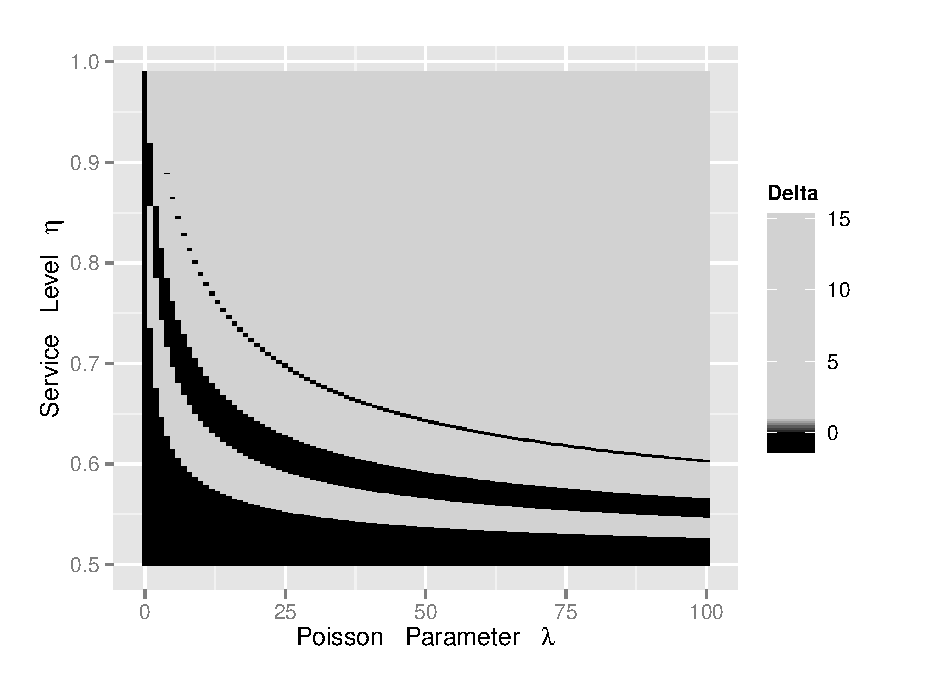
\includegraphics[width=15cm]{ShiXiao.eps}
\caption{泊松分布下的改进失效区间图示}
\label{fig:泊松分布下的改进失效区间图示}
\end{figure}

图\ref{fig:泊松分布下的改进失效区间图示}中每个点的位置代表一种$(\lambda,\eta)$组合,每个点的颜色代表该处的$\Delta$值。如果$\Delta\leq0$,则该点为黑色;如果$\Delta>0$,则该点为浅灰色。因此,图中的黑色区域代表发生改进失效的区域,灰色区域代表改进有效果的区域。

由于泊松分布的离散性,图\ref{fig:泊松分布下的改进失效区间图示}中的黑色区域边缘存在锯齿,甚至是断断续续的。从这幅图形中,我们能够得到很多有效的信息。

首先,它验证了前两节证明的一些论断。作为右偏斜分布的泊松分布,在服务水平大于0.5的某个区间内,确实出现了改进失效的一片区域;另外,当$\lambda\to0$时,黑色区域的延伸趋势也验证了上一节的论断,即不存在“不会发生改进失效的服务水平”。

其次,黑色区域在横轴方向的变化趋势告诉我们,需求量越大,发生改进失效的服务水平区间就越小,也就是说越不容易发生改进失效。当$\lambda$增大到一定程度时,泊松分布会趋近于正态分布。我们已经了解到,正态分布在$\eta>0.5$的时候是不会出现改进失效的。因此,随着$\lambda$的增长,黑色区域会越来越小,最终小到可以忽略的程度。结合上一节中伯努利分布的讨论可以看出,对于右偏斜的需求分布,偏斜程度越大,越可能发生改进失效。

最后,黑色区域在纵轴方向的变化趋势显示,服务水平越高,发生改进失效的区域越少。也就是说,这样的改进方法对于服务水平高的企业是有利的。虽然理论上不存在“不会发生改进失效的服务水平”,但是如果已经知道了需求的参数$\lambda$的一个确定的下限,就能够指出一个对应的服务水平的安全线,使得服务水平高于这个安全线时不可能发生改进失效。












\subsection{第二类服务水平与改进失效}

到目前为止,我们在提到服务水平时,都是指第一类服务水平,即得到满足的订单数占总订单数的比例。在实际生产中,也有一些企业采用第二类服务水平作为库存的制定标准。第二类服务水平是指得到满足的需求量占总需求量的比例。如果库存不足以满足需求,就从需求中减去现有的全部库存,剩余的量才作为未满足的需求量。下面我们将证明,如果改进前后都以相同的第二类服务水平作为制定库存的标准,则不可能发生改进失效。

我们知道,发生改进失效的判定标准是“服务水平不变的情况下,改进后的总库存大于改进前的总库存”。事实上,因为服务水平是随库存增加而单调增加的,因此上述判定标准等价于“总库存不变的情况下,改进后的服务水平低于改进前的服务水平”。所以,如果保持改进前后库存总量不变,只需证明改进后的第二类服务水平不可能低于改进前的第二类服务水平即可。

设两种成品的需求$D_1$、$D_2$相互独立,概率密度函数分别为$f_1(x_1)$和$f_2(x_2)$。企业的服务水平(第二类服务水平)为$\eta$。该服务水平下,两种成品的库存分别为$\xi_1$和$\xi_2$。根据第二类服务水平的定义,得到满足的需求量与总需求量之比的期望值为第二类服务水平。两种成品得到满足的需求量分别为$\min(x_1,\xi_1)$和$\min(x_2,\xi_2)$,因此有
\[
\eta = \int_{-\infty}^{+\infty}\frac{\min(x_1,\xi_1)}{x_1}f(x_1)\dif x_1 = \int_{-\infty}^{+\infty}\frac{\min(x_2,\xi_2)}{x_2}f(x_2)\dif x_2
\]

考虑两种成品需求的联合分布$f(x_1,x_2)$。由于需求是相互独立的,因此有$f(x_1,x_2)=f(x_1)f(x_2)$。将两种成品看做一个整体,则得到满足的需求量为$\min(x_1,\xi_1)+\min(x_2,\xi_2)$,总需求量为$x_1+x_2$。因为它们各自的服务水平都是$\eta$,所以综合服务水平也是$\eta$。因此有
\begin{equation}
\eta = \int_{-\infty}^{+\infty}\int_{-\infty}^{+\infty}\frac{\min(x_1,\xi_1)+\min(x_2,\xi_2)}{x_1+x_2}f(x_1)f(x_2)\dif x_1 \dif x_2
\label{eq:合并前第二类服务水平}
\end{equation}

现将两种成品库存合并到在制品库存,保持总量不变,即合并后的库存为$\xi=\xi_1+\xi_2$。合并后的服务水平为$\eta'$。合并后的总需求量为$x_1+x_2$,其中得到满足的需求量为$\min(x_1+x_2,\xi_1+\xi_2)$,因此合并后的服务水平为
\begin{equation}
\eta' = \int_{-\infty}^{+\infty}\int_{-\infty}^{+\infty}\frac{\min(x_1+x_2,\xi_1+\xi_2)}{x_1+x_2}f(x_1)f(x_2)\dif x_1 \dif x_2
\label{eq:合并后第二类服务水平}
\end{equation}

为了比较$\eta$和$\eta'$的大小,我们先证明$\min(x_1,\xi_1)+\min(x_2,\xi_2)\leq\min(x_1+x_2,\xi_1+\xi_2)$。设$m_1=\min(x_1,\xi_1)$,$m_2=\min(x_2,\xi_2)$,则有$m_1\leq x_1$,$m_1\leq\xi_1$,$m_2\leq x_2$,$m_2\leq\xi_2$。因此$x_1+x_2\geq m_1+m_2$,$\xi_1+\xi_2\geq m_1+m_2$。由此可证
\begin{align}
\min(x_1+x_2,\xi_1+\xi_2) &\geq \min(m_1+m_2,m_1+m_2) \notag\\
&= m_1+m_2 \notag\\
&= \min(x_1,\xi_1)+\min(x_2,\xi_2)
\label{eq:局部放缩_第二类服务水平}
\end{align}

将不等式\ref{eq:局部放缩_第二类服务水平}代入公式\ref{eq:合并前第二类服务水平}和\ref{eq:合并后第二类服务水平}中,就能比较$\eta$和$\eta'$的大小,具体过程如下:

\begin{align}
\eta' &= \int_{-\infty}^{+\infty}\int_{-\infty}^{+\infty}\frac{\min(x_1+x_2,\xi_1+\xi_2)}{x_1+x_2}f(x_1)f(x_2)\dif x_1 \dif x_2 \notag\\
&\geq \int_{-\infty}^{+\infty}\int_{-\infty}^{+\infty}\frac{\min(x_1,\xi_1)+\min(x_2,\xi_2)}{x_1+x_2}f(x_1)f(x_2)\dif x_1 \dif x_2 \notag\\
&= \eta
\label{eq:比较改进前后第二类服务水平}
\end{align}

由公式\ref{eq:比较改进前后第二类服务水平}可知,总库存保持不变的情况下,改进后的第二类服务水平不低于改进前的第二类服务水平。因此,保持第二类服务水平不变的情况下,改进后的库存不会大于改进前的库存。

至此,我们证明了本小节开头提出的观点,即“如果改进前后都以相同的第二类服务水平作为制定库存的标准,则不可能发生改进失效”。因此,对于使用第二类服务水平作为库存制定标准的企业来说,这样的改进是值得考虑的。












\section{避免改进失效}

通过本章的探讨,我们初步了解了改进失效现象的影响因素和具体表现。作为对本章的一个总结,我们在此简单归纳各种参数对改进失效的影响,作为企业改进前需要考虑的因素:

\begin{enumerate}
\item 如果需求服从正态分布,只需保证企业的服务水平大于0.5,即可避免改进失效;
\item 如果需求服从对称稳定分布,需要保证决定分布陡峭程度的参数$\alpha$的值在$(1,2]$区间内,才能避免改进失效;
\item 如果需求服从右偏斜的分布,需要关注需求分布的偏斜程度和企业的服务水平。分布的偏斜程度越大,,越可能发生改进失效;企业的服务水平越低,越可能发生改进失效。
\end{enumerate}

总而言之,企业做出改进决策之前,首先需要考虑的就是需求分布的特点,其次需要检查自身的服务水平在这个需求分布下有无改进失效的可能。





















